\clearpage
\slidetitle{Réseaux et neurones}

\begin{slide}

\begin{itemize}

	\item \textbf{Neurone:} associe à un vecteur $x = (x_1, \ldots, x_m)$ une sortie scalaire $\varphi(x)$, entrées pondérées par un \textit{poids} $p_i$ puis composition par une \textit{fonction d'activation} $f$ translatée par un \textit{biais} $b$.
	\begin{equation*}
		\varphi(x) = f (\sum_{i=1}^m p_i x_i - b) 
	\end{equation*}

	\item Fonction d'activation usuelle : $f(x) = \frac{1}{1 + \mathrm{e}^{-x}}$.

	\begin{figure}[h!]
	\centering
	\includegraphics[width=0.8\linewidth]{schemas/sigmoide.pdf}
	\end{figure}

\end{itemize}

\end{slide}

\clearpage
\slidetitle{Réseaux et neurones}

\begin{slide}

\begin{itemize}

	\item \textbf{Réseau:} application de $\mathbb{R}^p$ dans $\mathbb{R}^q$, modélisée par des couches de neurones.

	\item \textbf{Organisation en couches:} l'ensemble des sorties scalaires des neurones de la couche $c$ notées $\neurone{i}{c}$ sert d'entrée aux neurones de la couche $c+1$:
	\begin{equation*}
		\neurone{j}{c+1} = f ( \sum_{i=1}^{\lc{c}} \poids{i}{j}{c+1} \neurone{i}{c} ) = f( \nps{j}{c+1} ).
	\end{equation*}

\end{itemize}

\begin{figure}[!h]

	\centering

	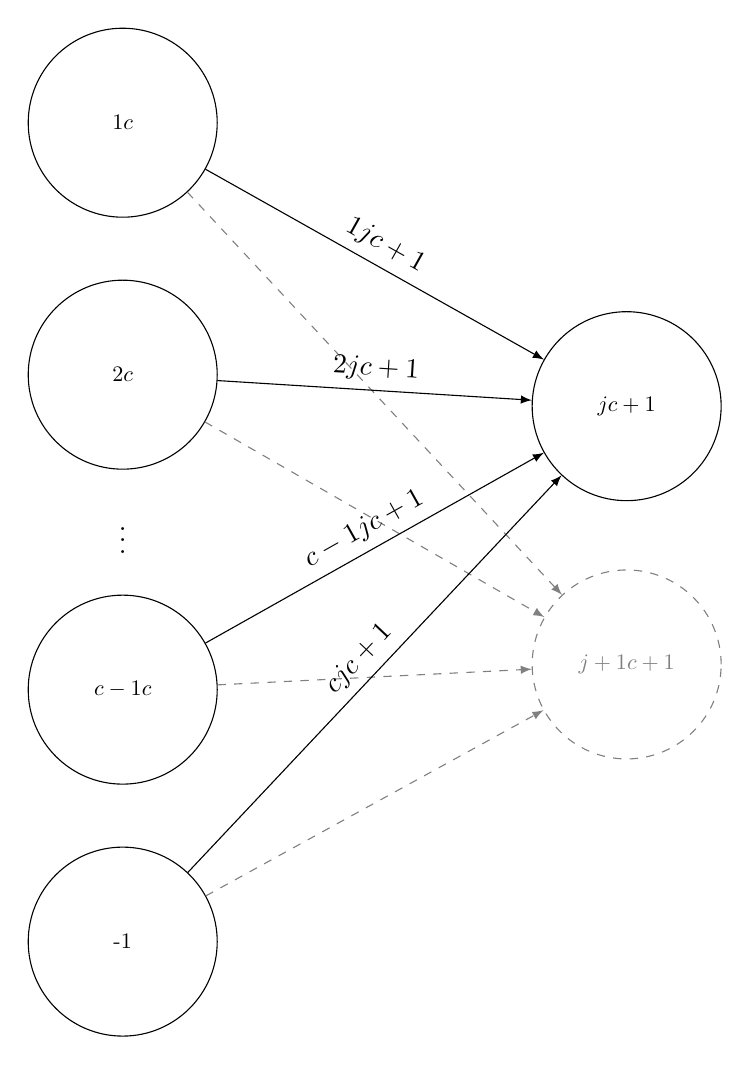
\begin{tikzpicture}[font=\normalsize, scale=0.8, x=1cm, y=1cm]

		\tikzstyle{neurone}=[draw, transform shape, circle, minimum size=3cm]
		\tikzstyle{fleche}=[->, >=latex]
		\tikzstyle{gris}=[dashed, gray]
		\tikzstyle{poids}=[midway, sloped, above]

		\node[neurone] (x1) at (0, 13) {$\neurone{1}{c}$};
		\node[neurone] (x2) at (0, 9) {$\neurone{2}{c}$};
		\draw (0, 6.5) node {\vdots};
		\node[neurone] (xk) at (0, 4) {$\neurone{\lc{c}-1}{c}$};
		\node[neurone] (biais) at (0, 0) {-1};
		\node[neurone] (xj) at (8, 8.5) {$\neurone{j}{c+1}$};
		\node[neurone, gris] (xj+1) at (8, 4.4) {$\neurone{j+1}{c+1}$};

		\draw[fleche, gris] (x1) -- (xj+1) node[poids] {};
		\draw[fleche, gris] (x2) -- (xj+1) node[poids] {};
		\draw[fleche, gris] (xk) -- (xj+1) node[poids] {};
		\draw[fleche, gris] (biais) -- (xj+1) node[poids] {};
		\draw[fleche] (x1) -- (xj) node[poids] {$\poids{1}{j}{c+1}$};
		\draw[fleche] (x2) -- (xj) node[poids] {$\poids{2}{j}{c+1}$};
		\draw[fleche] (xk) -- (xj) node[poids] {$\poids{\lc{c}-1}{j}{c+1}$};
		\draw[fleche] (biais) -- (xj) node[poids] {$\poids{\lc{c}}{j}{c+1}$};

	\end{tikzpicture}

\end{figure}

\end{slide}